\documentclass{article}
\usepackage[utf8]{inputenc}
\usepackage{geometry}
\usepackage{amsmath}
\usepackage{amssymb}
\usepackage{enumitem}
\usepackage{graphicx}
\graphicspath{ {../images/} }

\geometry{letterpaper, margin=1in}

\begin{document}

\begin{center}
    {\LARGE EE114 - Homework 1} \\[0.5cm]
    Name: Kaushik Vada \\[0.5cm]
    \today
\end{center}

\section*{Quiz 1.1}
A pizza at Gerlanda's is either regular ($R$) or Tuscan ($T$). In addition, each slice may have mushrooms ($M$) or onions ($O$) as described by the Venn diagram. For the sets specified below, shade the corresponding region of the Venn diagram.

\begin{center}
    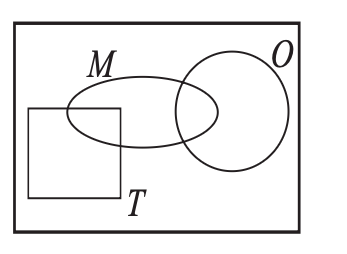
\includegraphics[width=0.2\textwidth]{quiz_1_1.png}
\end{center}

\begin{enumerate}[label=(\arabic*)]
    \item $R$ \\ \textbf{Solution:} Shade the circle $R$.
    \item $M \cup O$ \\ \textbf{Solution:} Shade the union of circles $M$ and $O$.
    \item $M \cap O$ \\ \textbf{Solution:} Shade the intersection of circles $M$ and $O$.
    \item $R \cup M$ \\ \textbf{Solution:} Shade values in either $R$ or $M$ (their union).
    \item $R \cap M$ \\ \textbf{Solution:} Shade the intersection of $R$ and $M$.
    \item $T^c - M$ \\ \textbf{Solution:} $T^c$ represents everything not in $T$, which corresponds to $R$. Then subtract $M$. Shade the region of $R$ that does not overlap with $M$.
\end{enumerate}

\section*{Problem 1.1.1}
For Gerlanda's pizza in Quiz 1.1, answer these questions:
\begin{enumerate}[label=(\alph*)]
    \item Are $T$ and $M$ mutually exclusive? \\
    \textbf{Solution:} No. A Tuscan pizza can have mushrooms. The intersection $T \cap M$ is not empty.
    \item Are $R, T,$ and $M$ collectively exhaustive? \\
    \textbf{Solution:} Yes. Since pizza types are $\{R, T\}$, $R \cup T = S$.  Thus $R \cup T \cup M = S$. They cover the entire sample space.
    \item Are $T$ and $O$ mutually exclusive? State this condition in words. \\
    \textbf{Solution:} No. A Tuscan pizza can have onions. Condition: $T \cap O = \emptyset$ (false here).
    \item Does Gerlanda's make Tuscan pizzas with mushrooms and onions? \\
    \textbf{Solution:} Yes, provided the intersection $T \cap M \cap O$ is non-empty.
    \item Does Gerlanda's make regular pizzas that have neither mushrooms nor onions? \\
    \textbf{Solution:} Yes, this is the region $R \cap M^c \cap O^c$.
\end{enumerate}

\newpage

\section*{Problem 1.2.1}
A fax transmission can take place at any of three speeds depending on the condition of the phone connection between the two fax machines. The speeds are high ($h$) at 14,400 b/s, medium ($m$) at 9600 b/s, and low ($l$) at 4800 b/s. In response to requests for information, a company sends either short faxes of two ($t$) pages, or long faxes of four ($f$) pages. Consider the experiment of monitoring a fax transmission and observing the transmission speed and length. An observation is a two-letter word, for example, a high-speed, two-page fax is $ht$.

\begin{enumerate}[label=(\alph*)]
    \item What is the sample space of the experiment? \\
    \textbf{Solution:} $S = \{ht, hf, mt, mf, lt, lf\}$.
    \item Let $A_1$ be the event ``medium-speed fax.'' What are the outcomes in $A_1$? \\
    \textbf{Solution:} $A_1 = \{mt, mf\}$.
    \item Let $A_2$ be the event ``short (two-page) fax.'' What are the outcomes in $A_2$? \\
    \textbf{Solution:} $A_2 = \{ht, mt, lt\}$.
    \item Let $A_3$ be the event ``high-speed fax or low-speed fax.'' What are the outcomes in $A_3$? \\
    \textbf{Solution:} $A_3 = \{ht, hf, lt, lf\}$.
    \item Are $A_1, A_2,$ and $A_3$ mutually exclusive? \\
    \textbf{Solution:} No. $A_1 \cap A_2 = \{mt\} \neq \emptyset$.
    \item Are $A_1, A_2,$ and $A_3$ collectively exhaustive? \\
    \textbf{Solution:} Yes. $A_1 \cup A_2 \cup A_3 = \{mt, mf, ht, lt, hf, lf\} = S$.
\end{enumerate}

\newpage

\section*{Problem 1.2.2}
An integrated circuit factory has three machines $X, Y,$ and $Z$. Test one integrated circuit produced by each machine. Either a circuit is acceptable ($a$) or it fails ($f$). An observation is a sequence of three test results corresponding to the circuits from machines $X, Y,$ and $Z$, respectively. For example, $aaf$ is the observation that the circuits from $X$ and $Y$ pass the test and the circuit from $Z$ fails the test.

\begin{enumerate}[label=(\alph*)]
    \item What are the elements of the sample space of this experiment? \\
    \textbf{Solution:} $S = \{aaa, aaf, afa, aff, faa, faf, ffa, fff\}$.
    \item What are the elements of the sets
    \[ Z_F = \{ \text{circuit from } Z \text{ fails} \}, \]
    \[ X_A = \{ \text{circuit from } X \text{ is acceptable} \}. \]
    \textbf{Solution:} \\
    $Z_F = \{aaf, aff, faf, fff\}$ \\
    $X_A = \{aaa, aaf, afa, aff\}$
    \item Are $Z_F$ and $X_A$ mutually exclusive? \\
    \textbf{Solution:} No. $Z_F \cap X_A = \{aaf, aff\} \neq \emptyset$.
    \item Are $Z_F$ and $X_A$ collectively exhaustive? \\
    \textbf{Solution:} No. $Z_F \cup X_A = S \setminus \{faa, ffa\}$. It is missing elements where X fails and Z passes.
    \item What are the elements of the sets
    \[ C = \{ \text{more than one circuit acceptable} \}, \]
    \[ D = \{ \text{at least two circuits fail} \}. \]
    \textbf{Solution:} \\
    $C = \{ \text{2 or 3 'a's} \} = \{aaa, aaf, afa, faa\}$ \\
    $D = \{ \text{2 or 3 'f's} \} = \{aff, faf, ffa, fff\}$
    \item Are $C$ and $D$ mutually exclusive? \\
    \textbf{Solution:} Yes. $C$ contains outcomes with $\ge 2$ a's (thus $\le 1$ f), $D$ contains outcomes with $\ge 2$ f's. They cannot overlap.
    \item Are $C$ and $D$ collectively exhaustive? \\
    \textbf{Solution:} Yes. Any outcome has either $\le 1$ f (in $C$) or $\ge 2$ f (in $D$). They partition the space.
\end{enumerate}

\newpage

\section*{Problem 1.3.1}
Computer programs are classified by the length of the source code and by the execution time. Programs with more than 150 lines in the source code are big ($B$). Programs with $\le 150$ lines are little ($L$). Fast programs ($F$) run in less than 0.1 seconds. Slow programs ($W$) require at least 0.1 seconds. Monitor a program executed by a computer. Observe the length of the source code and the run time. The probability model for this experiment contains the following information: $P[LF] = 0.5$, $P[BF] = 0.2$, and $P[BW] = 0.2$. What is the sample space of the experiment? Calculate the following probabilities:

\begin{enumerate}[label=(\alph*)]
    \item $P[W]$ \\
    \textbf{Solution:} Given $P[LF]=0.5, P[BF]=0.2, P[BW]=0.2$. Sum of elementary events is 1. \\
    $P[LF]+P[LW]+P[BF]+P[BW]=1 \implies 0.5+P[LW]+0.2+0.2=1 \implies P[LW]=0.1$. \\
    $P[W] = P[LW] + P[BW] = 0.1 + 0.2 = 0.3$.
    \item $P[B]$ \\
    \textbf{Solution:} $P[B] = P[BF] + P[BW] = 0.2 + 0.2 = 0.4$.
    \item $P[W \cup B]$ \\
    \textbf{Solution:} $P[W \cup B] = P[W] + P[B] - P[W \cap B]$. $W \cap B = BW$. \\
    So $P[W \cup B] = 0.3 + 0.4 - 0.2 = 0.5$.
\end{enumerate}

\newpage

\section*{Problem 1.3.2}
There are two types of cellular phones, handheld phones ($H$) that you carry and mobile phones ($M$) that are mounted in vehicles. Phone calls can be classified by the traveling speed of the user as fast ($F$) or slow ($W$). Monitor a cellular phone call and observe the type of telephone and the speed of the user. The probability model for this experiment has the following information: $P[F] = 0.5$, $P[HF] = 0.2$, $P[MW] = 0.1$. What is the sample space of the experiment? Calculate the following probabilities:

\begin{enumerate}[label=(\alph*)]
    \item $P[W]$ \\
    \textbf{Solution:} $P[W] = 1 - P[F] = 1 - 0.5 = 0.5$.
    \item $P[MF]$ \\
    \textbf{Solution:} $P[F] = P[HF] + P[MF] \implies 0.5 = 0.2 + P[MF] \implies P[MF] = 0.3$.
    \item $P[H]$ \\
    \textbf{Solution:} First find $P[M]$. $P[M] = P[MF] + P[MW] = 0.3 + 0.1 = 0.4$. \\
    Then $P[H] = 1 - P[M] = 1 - 0.4 = 0.6$. (Check: $P[H] = P[HF] + (P[W]-P[MW]) = 0.2 + (0.5-0.1) = 0.6$).
\end{enumerate}

\newpage

\section*{Problem 1.4.1}
Mobile telephones perform \textit{handoffs} as they move from cell to cell. During a call, a telephone either performs zero handoffs ($H_0$), one handoff ($H_1$), or more than one handoff ($H_2$). In addition, each call is either long ($L$), if it lasts more than three minutes, or brief ($B$). The following table describes the probabilities of the possible types of calls.

\begin{center}
\begin{tabular}{c|ccc}
 & $H_0$ & $H_1$ & $H_2$ \\
\hline
$L$ & 0.1 & 0.1 & 0.2 \\
$B$ & 0.4 & 0.1 & 0.1
\end{tabular}
\end{center}

\noindent
What is the probability $P[H_0]$ that a phone makes no handoffs? \\
\textbf{Solution:} $P[H_0] = 0.1 + 0.4 = 0.5$.

\noindent
What is the probability a call is brief? \\
\textbf{Solution:} $P[B] = 0.4 + 0.1 + 0.1 = 0.6$.

\noindent
What is the probability a call is long or there are at least two handoffs? \\
\textbf{Solution:} $P[L \cup H_2] = P[L] + P[H_2] - P[L \cap H_2]$. \\
$P[L] = 0.1+0.1+0.2 = 0.4$. \\
$P[H_2] = 0.2+0.1 = 0.3$. \\
$P[L \cap H_2] = 0.2$. \\
$P[L \cup H_2] = 0.4 + 0.3 - 0.2 = 0.5$.

\newpage

\section*{Problem 1.4.2}
For the telephone usage model of Example 1.14, let $B_m$ denote the event that a call is billed for $m$ minutes. To generate a phone bill, observe the duration of the call in integer minutes (rounding up). Charge for $M$ minutes $M = 1, 2, 3, \dots$ if the exact duration $T$ is $M - 1 < t \le M$. A more complete probability model shows that for $m = 1, 2, \dots$ the probability of each event $B_m$ is
\[ P[B_m] = \alpha(1 - \alpha)^{m-1} \]
where $\alpha = 1 - (0.57)^{1/3} = 0.171$.

\begin{enumerate}[label=(\alph*)]
    \item Classify a call as long, $L$, if the call lasts more than three minutes. What is $P[L]$? \\
    \textbf{Solution:} A call lasts $>3$ minutes if it is billed for $m \ge 4$. \\
    $P[L] = \sum_{m=4}^\infty P[B_m] = \sum_{m=4}^\infty \alpha(1-\alpha)^{m-1}$. \\
    Let $k=m-1$, sum is $\sum_{k=3}^\infty \alpha(1-\alpha)^k = \frac{\alpha(1-\alpha)^3}{1-(1-\alpha)} = (1-\alpha)^3$. \\
    Given $\alpha = 1 - 0.57^{1/3}$, we have $1-\alpha = 0.57^{1/3}$. \\
    So $P[L] = (0.57^{1/3})^3 = 0.57$.
    \item What is the probability that a call will be billed for nine minutes or less? \\
    \textbf{Solution:} $P[M \le 9] = 1 - P[M > 9]$. \\
    $M > 9 \implies M \ge 10$. \\
    $P[M \ge 10] = \sum_{m=10}^\infty P[B_m] = (1-\alpha)^9$. \\
    Using $1-\alpha = 0.57^{1/3}$, $P[M \ge 10] = (0.57^{1/3})^9 = 0.57^3 \approx 0.185$. \\
    $P[M \le 9] = 1 - 0.185 = 0.815$.
\end{enumerate}

\newpage

\section*{Problem 1.4.3}
The basic rules of genetics were discovered in mid-1800s by Mendel, who found that each characteristic of a pea plant, such as whether the seeds were green or yellow, is determined by two genes, one from each parent. Each gene is either dominant $d$ or recessive $r$. Mendel's experiment is to select a plant and observe whether the genes are both dominant $d$, both recessive $r$, or one of each (hybrid) $h$. In his pea plants, Mendel found that yellow seeds were a dominant trait over green seeds. A $yy$ pea with two yellow genes has yellow seeds; a $gg$ pea with two recessive genes has green seeds; a hybrid $gy$ or $yg$ pea has yellow seeds. In one of Mendel's experiments, he started with a parental generation in which half the pea plants were $yy$ and half the plants were $gg$. The two groups were crossbred so that each pea plant in the first generation was $gy$. In the second generation, each pea plant was equally likely to inherit a $y$ or a $g$ gene from each first generation parent. What is the probability $P[Y]$ that a randomly chosen pea plant in the second generation has yellow seeds? \\
\textbf{Solution:} \\
Start: $P(yy)=0.5, P(gg)=0.5$. \\
F1: All $gy$. \\
F2: Cross $gy \times gy$. \\
Offspring genotypes: $yy, yg, gy, gg$ each with probability $1/4$. \\
Yellow seeds occur for $yy, yg, gy$. \\
$P[Y] = P(yy) + P(yg) + P(gy) = 1/4 + 1/4 + 1/4 = 3/4 = 0.75$.

\newpage

\section*{Problem 1.4.4}
Use Theorem 1.7 to prove the following facts:
\begin{enumerate}[label=(\alph*)]
    \item $P[A \cup B] \ge P[A]$ \\
    \textbf{Proof:} $A \subseteq A \cup B$. By Monotonicity Axiom, $P[A] \le P[A \cup B]$.
    \item $P[A \cup B] \ge P[B]$ \\
    \textbf{Proof:} $B \subseteq A \cup B$. By Monotonicity Axiom, $P[B] \le P[A \cup B]$.
    \item $P[A \cap B] \le P[A]$ \\
    \textbf{Proof:} $A \cap B \subseteq A$. By Monotonicity Axiom, $P[A \cap B] \le P[A]$.
    \item $P[A \cap B] \le P[B]$ \\
    \textbf{Proof:} $A \cap B \subseteq B$. By Monotonicity Axiom, $P[A \cap B] \le P[B]$.
\end{enumerate}

\newpage

\section*{Problem 1.4.5}
Use Theorem 1.7 to prove by induction the \textit{union bound}: For any collection of events $A_1, \dots, A_n$,
\[ P[A_1 \cup A_2 \cup \dots \cup A_n] \le \sum_{i=1}^n P[A_i]. \]
\textbf{Proof:} \\
\textit{Base Case ($n=2$):} $P(A_1 \cup A_2) = P(A_1) + P(A_2) - P(A_1 \cap A_2)$. Since $P(A_1 \cap A_2) \ge 0$, $P(A_1 \cup A_2) \le P(A_1) + P(A_2)$. \\
\textit{Induction Step:} Assume true for $n=k$. \\
$P(\cup_{i=1}^{k+1} A_i) = P( (\cup_{i=1}^k A_i) \cup A_{k+1} )$. \\
By base case, this is $\le P(\cup_{i=1}^k A_i) + P(A_{k+1})$. \\
By inductive hypothesis, $P(\cup_{i=1}^k A_i) \le \sum_{i=1}^k P(A_i)$. \\
Substituting this in, $P(\cup_{i=1}^{k+1} A_i) \le \sum_{i=1}^k P(A_i) + P(A_{k+1}) = \sum_{i=1}^{k+1} P(A_i)$. \\
The statement holds for all $n$.

\end{document}